\documentclass[6pt]{ctexbook}
\input{~/latex/book-preamble-chinese.tex}

\begin{document}

\newcommand{\mytitle}{Git}
\newcommand{\firstcreated}{Mar 16, 2023}

\begin{titlepage}

\newcommand{\HRule}{\rule{\linewidth}{0.5mm}} % Defines a new command for the horizontal lines, change thickness here

\center                         % Center everything on the page
 
%----------------------------------------------------------------------------------------
%	HEADING SECTIONS
%----------------------------------------------------------------------------------------


\includegraphics[width=0.5\textwidth]{logo}\\[1cm] % Include a department/university logo - this will require the graphicx package

%----------------------------------------------------------------------------------------
%	TITLE SECTION
%----------------------------------------------------------------------------------------

\HRule\\[0.4cm]
{ \huge \bfseries \mytitle}\\[0.4cm] % Title of your document
\HRule\\[1.5cm]
 
%----------------------------------------------------------------------------------------
%	AUTHOR SECTION
%----------------------------------------------------------------------------------------

\begin{minipage}{0.4\textwidth}
\begin{center} \large
Mingming \textsc{Li}\\ % Your name
\end{center}

\end{minipage}\\[2cm]


%----------------------------------------------------------------------------------------
%	DATE SECTION
% ----------------------------------------------------------------------------------------
\vfill
{\large First Created: \firstcreated}\\
{\large Last Modified: \today}\\[2cm] % Date, change the \today to a set date if you want to be precise



\end{titlepage}


%%% Local Variables:
%%% mode: latex
%%% Tex-master: "git"
%%% End:
\frontmatter{}
\tableofcontents{}
% \listoftables{}
% \listoffigures{}
\mainmatter{}


\chapter{前言}


语言的主要作用是交流。如果我们独自生活在这个世界上,我们其实是不需要语
言的,我们对世界的认知以六感(图像,声音,味道,气味,触感和综合历史五
感记忆和现在场的影响形成的对未来的感觉)的形式存储在我们的头脑中。

语言不是帮助我们认知世界的,但语言的发展有利于大脑的开发,人是因为其社
会属性才称之为人的,没有社会属性,更确切的称之为动物。


因为语言的主要作用是交流,用于交流的,其实是听说,读写是为了扩大交流的
范围。历史上也是先出现的语言,后出现的文字,我们小时候也是,我们先学会
的说话,之后学会的写字。




法语的学习分为:听说读写。


\section{听}


我们听到一段声音,我们尝试去理解这段声音,这个过程类似决策树。
我们要做的第一个决策是声音的划分,我们首先将声音划分为多个音节,这是一个有反馈的划分,
我们在头脑中寻找和第一个音节相对应的词语,当我们没有找到的情况下,我们
尝试增加一个或者多个,然后再去寻找对应的词语,对应的词语可能有很多,我
们需要从中筛选出一个选择,帮助做出这个决策是语境(表情,下文,语气等
等),所以听力的基础是声音和词语的联系,需要根据声音筛选词语,词汇量的
多寡影响决策树分支的完备性。

一段声音中,每个音节的权重并不一定是相同的,一般权重大的是名词,动词,
代词和形容词所对应的声音,它们承载主体的信息。


我们去理解一段话,刚开始是经过思考的,有意识的,经过不断的重复和联系,
最终会建立不经过思考的,无意识的声音和词语的链接。

听的训练:强化声音和词语的链接,这个过程是通过不断重复实现的。


\section{说}

说一定程度上是身体的记忆,记忆的部分为口,舌,肺,腹。
当我们想要表达某个意思,我们根据头脑中存储的词语,去链接对应的发音,
结果我们的身体发出对应的声音。

我们首先需要身体记忆每个音标的发音,并形成身体记忆。下一步是记忆音标组
合成音节,最后是音节之间的过渡。我们说的时候磕磕巴巴,有一下原因:
\begin{itemize}
\item 我们不知道某个词语。
\item 我们知道某个词语,但词语和声音的链接不牢固,需要话时间进行链接。
\item 我们的链接很牢固,比如一听就知道,但说的不顺,因为未形成身体记忆,
  需要化时间去调节肌肉来发出对应的声音。
\end{itemize}

说的训练:强化身体记忆和词语的链接,这个过程是通过不同重复实现的。



\section{读}

读是看到一个符号,知道它的意思。读的基础是符号对词语意思的链接。

汉字是二维空间上的符号,是一种象形文字,法语(英语)是一维空间上的符号。记忆汉字可以
用偏旁部首来帮助记忆,然后因为一维的缘故,记忆法语单词就抽象了很多,
少了想象的空间。有两个解决途径,1. 人为刻意加入想象力。 2. 使用前缀,
词根,后缀和组合次法,类比汉字中的偏旁部首,只是少了形象部分。



\section{写}

写和读类似,也是符号和意思的链接,但这个比读困难,因为读是在现有符号下,
对符号和意思链接的回忆,而读则是没有任何帮助下,对符号和意思链接的回忆。





\section{语法}

在有链接的基础后,思维的表达涉及到表达的习惯,每个国家的人思维表达的习
惯都不同,进而形成了不同的语法,学习语法其实是学习语言的思维方式。







%%% Local Variables:
%%% mode: latex
%%% TeX-master: "french"
%%% End:


% \part{准备}

% 
\chapter{法语输入法}

\section{添加法语输入法}


MacBook带有法语输入法,添加输入法的方式为:
\begin{enumerate}
\item 点击左上角苹果图标
\item 选择system preference
\item 选择keyboard
\item 选择input source
\item 点击加号,添加法语输入法
\end{enumerate}

\section{法语输入法的使用}
法语键盘如图\ref{fig:french-input}所示:
\begin{figure}[!ht]
  \centering
  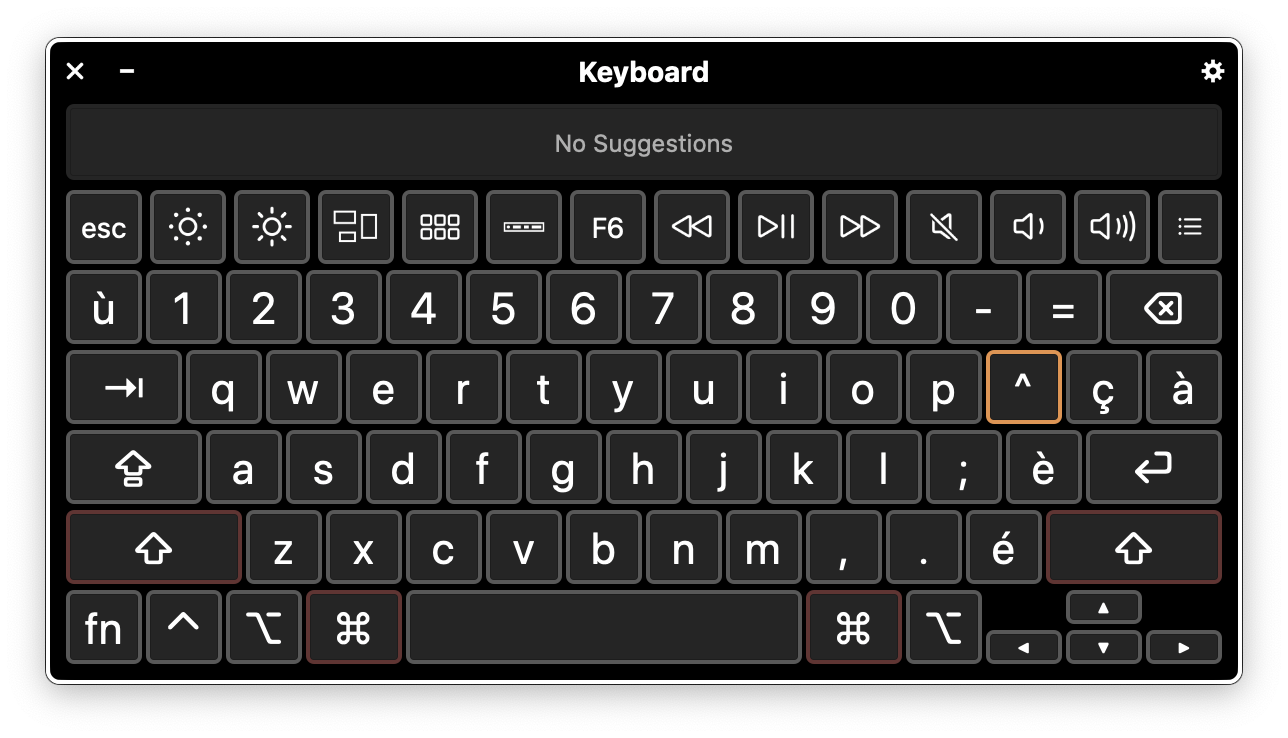
\includegraphics[width=\textwidth]{pic/french-input.png}
  \caption{法语键盘}
  \label{fig:french-input}
\end{figure}




\part{发音}

\chapter{音标}



\section{元音}
元音表示响亮的音。

\begin{description}
\item[[a]] là \textipa{[la]} 那里,这里
\item[[e]] dé \textipa{[de]} 骰子
\item[[i]] vie \textipa{[vi]} 生活
\item[[o]] dos \textipa{[do]} 背,背部
\item[[u]] fou \textipa{[fu]} 疯子,狂人
\item[[y]] tu \textipa{[ty]} 你
\item[\textipa{[\o]}] deux \textipa{[d\o]} 二,第二
\item[\textipa{[\oe]}] leur \textipa{[l\oe r]} 他们的,她们的,它们的
\item[\textipa{[O]}] port \textipa{[pOr]} 港口,携带
\item[\textipa{[@]}] me \textipa{[m@]} 我
\item[\textipa{[E]}] pelle \textipa{[pEl]} 铲
\end{description}

\subsection{辅音}

\subsubsection{清辅音}

\begin{description}
\item[[p]] nappe \textipa{[nap]} 桌布
\item[[t]] têle \textipa{[tele]} 电视
\item[[k]] lac \textipa{[lak]} 湖泊
\item[[f]] face \textipa{[fas]} 脸
\item[[s]] sel \textipa{[sel]} 盐
\item[\textipa{[S]}] chute \textipa{[Syt]} 跌落,倒塌
\end{description}

\subsubsection{浊辅音}

\begin{description}
\item[[b]] bar \textipa{[bar]} 酒吧
\item[[d]] double \textipa{[dubl]} 两倍的
\item[[g]] gare \textipa{[gar]} 泊船站,火车站,地铁站,飞机场
\item[[v]] vie \textipa{[vi]} 生活
\item[[z]] case \textipa{[kaz]} 茅屋,格子
\item[\textipa{[Z]}] juste \textipa{[Zyst]} 公平的,公正的
\end{description}

\subsubsection{鼻音}

\begin{description}
\item[[l]] lin \textipa{[l\~e]} 亚麻,亚麻布
\item[[m]] mur \textipa{[myr]} 墙壁,围墙
\item[[n]] nuire \textipa{[n4ir]} 损害,危害,妨碍

\end{description}


\subsubsection{其他}

\begin{description}
\item[[r]] port \textipa{[pOr]} 港口,携带
\item[\textipa{[\textltailn]}] ligne \textipa{[li\textltailn]} 线,界限,路线,标志线
\end{description}



\subsection{半元音}

\begin{description}
\item[[j]] pinao \textipa{[pjano]} 钢琴
\item[\textipa{[4]}] puis \textipa{[p4i]} 然后,接着,再者
\item[[w]] moi \textipa{[mwa]} 我
\end{description}

\section{鼻元音}

\begin{description}
\item[\textipa{[\~a]}] pente \textipa{[p\~at]} 斜坡,倾斜,坡度
\item[\textipa{[\~O]}] tombe \textipa{[t\~ob]} 墓地,墓穴,墓碑
\item[\textipa{[\~e]}] simple \textipa{[s\~epl]} 简单的,单一的
\item[\textipa{[\~\oe]}] un \textipa{[\~\oe]} 一个,一次
\end{description}



%%% Local Variables:
%%% mode: latex
%%% TeX-master: "french"
%%% End:

\chapter{字母表}

\begin{table}[!ht]
  \centering
  \begin{tabular}{lll}
    \toprule[1.5pt]
    A & a & \textipa{[a]} \\
    B & b & \textipa{[be]} \\
    C & c & \textipa{[se]} \\
    D & d & \textipa{[de]} \\
    E & e & \textipa{[@]} \\
    F & f & \textipa{[Ef]} \\
    G & g & \textipa{[Ze]} \\
    H & h & \textipa{[aS]} \\
    I & i & \textipa{[i]} \\
    J & j & \textipa{[Zi]} \\
    K & k & \textipa{[ka]} \\
    L & l & \textipa{[El]} \\
    M & m & \textipa{[Em]} \\
    N & n & \textipa{[En]} \\
    O & o & \textipa{[o]} \\
    P & p & \textipa{[pe]} \\
    Q & q & \textipa{[ky]} \\
    R & r & \textipa{[Er]} \\
    S & s & \textipa{[Es]} \\
    T & t & \textipa{[te]} \\
    U & u & \textipa{[y]} \\
    V & v & \textipa{[ve]} \\
    W & w & \textipa{[dubl@ve]} \\
    X & x & \textipa{[iks]} \\
    Y & y & \textipa{[igrEk]} \\
    Z & z & \textipa{[zEd]} \\
    \bottomrule[1.5pt]
  \end{tabular}
  \caption{字母表}
\end{table}

\chapter{发音规则}

发音规则的意思是,绝大多数情况下,是按这个规律来的,但有少数例外的情况,
特别是外来词(比如从其他语言引进的词语)。


\section{单个字母在单词中的单一音}

字母组合大于字母,即,如果字母形成字母组合,则字母组合的发音规律优先。
\begin{table}[H]
  \centering
  \begin{tabular}{lll}
    \toprule[1.5pt]
    a & \textipa{[a]} & lama\textipa{[lama]}\\
    i & \textipa{[i]} & ni\textipa{[ni]}\\
    y & \textipa{[i]} & cyclone\textipa{[siklon]}\\
    u & \textipa{[y]} & unique\textipa{[ynik]}\\
    b & \textipa{[b]} & habit\textipa{[abi]}\\
    d & \textipa{[d]} & hardi\textipa{[ardi]}\\
    f & \textipa{[f]} & film\textipa{[film]}\\
    l & \textipa{[l]} & film\textipa{[film]}\\
    m & \textipa{[m]} & film\textipa{[film]}\\
    n & \textipa{[n]} & ni\textipa{[ni]}\\
    j & \textipa{[Z]} & jour\textipa{[Zur]}\\
    r & \textipa{[r]} & France\textipa{[fr\~as]}\\
    h & \textipa{[]} 不发音 & habit\textipa{[abi]} \\
    v & \textipa{[v]} & vie\textipa{[vi]}\\
    z & \textipa{[z]} & bizarre\textipa{[bizar]}\\
    q & \textipa{[k]} & coq\textipa{[kOk]} \\
    \bottomrule[1.5pt]
  \end{tabular}
  \caption{字母在单词中的发音}
\end{table}

\section{四大拼读规则}

\begin{enumerate}
\item e在词未不发音,除短小词外,短小词中发\textipa{[@]}。(le\textipa{[l@], te\textipa{[t@], de\textipa{[d@]}}})
\item 辅音字母在词末不发音,除cflr(长发丽人)。
\item h永不发音。
\item 两个相同的字母发一个音。
\end{enumerate}

\section{一个字母多个发音}

\subsection{c}
\begin{table}[H]
  \centering
  \begin{tabular}{lll}
    \toprule[1.5pt]
    \textipa{[s]} & 在e,i,y前 & ceci\textipa{[s@si]}, cycle\textipa{[sikl]} \\
    \textipa{[k]} & 不在e,i,y前 & car\textipa{[kar]}, lac\textipa{[lak]} \\
    \bottomrule[1.5pt]
  \end{tabular}
  \caption{c的发音}
\end{table}

\subsection{g}

\begin{table}[H]
  \centering
  \begin{tabular}{lll}
    \toprule[1.5pt]
    \textipa{[Z]} & 在e,i,y前 & girafe\textipa{[Ziraf]}, gel\textipa{[ZEl]} \\
    \textipa{[g]} & 不在e,i,y前 & gare\textipa{[gar]}, glace\textipa{[glas]} \\
    \textipa{[g]} & gu组合 & guerre\textipa{[gE:r]}, guide\textipa{[gid]} \\
    \bottomrule[1.5pt]
  \end{tabular}
  \caption{g的发音}
\end{table}

\subsection{o}

\begin{table}[H]
  \centering
  \begin{tabular}{lll}
    \toprule[1.5pt]
    \textipa{[O]} & 一般情况下 & porte\textipa{[pOrt]}, sport\textipa{[spOr]} \\
    \textipa{[o]} & 词末开音节 & mot\textipa{[mo]} \\
    \textipa{[o]} & \textipa{[z]}音前的o & rose\textipa{[roz]} \\
    \bottomrule[1.5pt]
  \end{tabular}
  \caption{o的发音}
\end{table}

\subsection{q}

\begin{table}[H]
  \centering
  \begin{tabular}{lll}
    \toprule[1.5pt]
    \textipa{[k]} & q在词尾 & coq\textipa{[kOk]} \\
    \textipa{[k]} & qu组合中 & qui\textipa{[ki]}, que\textipa{[k@]} \\
    \bottomrule[1.5pt]
  \end{tabular}
  \caption{q的发音}
\end{table}


\subsection{s}

\begin{table}[H]
  \centering
  \begin{tabular}{lll}
    \toprule[1.5pt]
    \textipa{[s]} & 大多数情况下 & si\textipa{[si]}, sel\textipa{[sEl]} \\
    \textipa{[z]} & s在两个元音字母中间 & rose\textipa{[roz]}, pose\textipa{[poz]} \\
    \bottomrule[1.5pt]
  \end{tabular}
  \caption{s的发音}
\end{table}

\subsection{w}

\begin{table}[H]
  \centering
  \begin{tabular}{lll}
    \toprule[1.5pt]
    \textipa{[w]} & 外来词 & wifi\textipa{[wifi]}, walt\textipa{[walt]} \\
    \textipa{[v]} & 一般情况下 & wagon\textipa{[vag\~o]} \\
    \bottomrule[1.5pt]
  \end{tabular}
  \caption{w的发音}
\end{table}

\subsection{x}

\begin{table}[H]
  \centering
  \begin{tabular}{lll}
    \toprule[1.5pt]
    \textipa{[s]} & 在极个别的词末 & six\textipa{[sis]}, dix\textipa{[dis]} \\
    \textipa{[Egz]} & ex+元音 & examiner\textipa{[Egzamine]}, exemple\textipa{[Egz\~apl]} \\
    \textipa{[Eks]} & ex+辅音 & excuse\textipa{[Ekskyz]} \\
    \textipa{[ks]} & x单独在词中 & taxi\textipa{[taksi]} \\
    \bottomrule[1.5pt]
  \end{tabular}
  \caption{x的发音}
\end{table}

\subsection{e}

\begin{table}[H]
  \centering
  \begin{tabular}{lll}
    \toprule[1.5pt]
    \textipa{[E]} & 在闭音节中 & sel\textipa{[sEl]}, mer\textipa{[mEr]}, merci\textipa{[mErsi]} \\
    \textipa{[@]} & 在开音节 & ceci\textipa{[s@si]}, sela\textipa{[s@la]} \\
    \textipa{[a]} & 在两个mm前 & femme\textipa{[fam]} \\
    \textipa{[e]} & -er, -ez字母组合在词尾 & aimer\textipa{[Eme]} \\
                  & -ez在单音节词尾 & mes, des, ses \\
    不发音 & 元辅e辅元 & samedi\textipa{[samdi]} \\
    \bottomrule[1.5pt]
  \end{tabular}
  \caption{e的发音}
\end{table}


\section{带字符的字母}


\begin{table}[H]
  \centering
  \begin{tabular}{lll}
    \toprule[1.5pt]
    à, â & \textipa{[a]} & là\textipa{[la]} \\
    é & \textipa{[e]} & passé\textipa{[pase]}\\
    è,ê,ë & \textipa{[E]} & près\textipa{[prE]}\\
    î,ï & \textipa{[i]} & île\textipa{[il]}, maïs\textipa{[mais]}\\
    ô & \textipa{[o]} & tôt\textipa{[to]}\\
    ç & \textipa{[s]} & français\textipa{[fr\~asEz]}\\
    ù,û & \textipa{[y]} & sûr\textipa{[syr]}\\
    \bottomrule[1.5pt]
  \end{tabular}
  \caption{带字符的字母}
\end{table}


\section{字母组合的发音}
一般指多个元音字母相连。

\begin{table}[H]
  \centering
  \begin{tabular}{p{0.2\columnwidth}p{0.1\columnwidth}p{0.5\columnwidth}}
    \toprule[1.5pt]
    ai, ei, ay, ey & \textipa{E} & faire\textipa{[fEr]}, clair\textipa{[klEr]}, Seine\textipa{[sEn]}, seize\textipa{[sEz]} \\
    \bottomrule[1.5pt]
  \end{tabular}
  \caption{ai, ei, ay, ey}
\end{table}

\begin{table}[H]
  \centering
  \begin{tabular}{p{0.2\columnwidth}p{0.1\columnwidth}p{0.5\columnwidth}}    
    \toprule[1.5pt]
    oi & \textipa{[wa]} & soir\textipa{[swar]}, voir\textipa{[vwar]} \\
    \bottomrule[1.5pt]
  \end{tabular}
  \caption{oi}
\end{table}

\begin{table}[H]
  \centering
  \begin{tabular}{p{0.2\columnwidth}p{0.1\columnwidth}p{0.5\columnwidth}}    
    \toprule[1.5pt]
    au, eau & \textipa{[o]} & auto\textipa{[odo]}, aussi\textipa{[osi]}, au\textipa{[o]}, beau\textipa{[bo]} \\
    \bottomrule[1.5pt]
  \end{tabular}
  \caption{au, eau}
\end{table}


\begin{table}[H]
  \centering
  \begin{tabular}{p{0.2\columnwidth}p{0.3\columnwidth}p{0.3\columnwidth}}
    \toprule[1.5pt]
    eu & 一般情况下发\textipa{[\o]} & bleu\textipa{[bl\o]},
                                      feu\textipa{[f\o]} \\
    & 在r前面发\textipa{\oe} & leur\textipa{[l\oe r]}, coeur\textipa{k\oe r]} \\
    \bottomrule[1.5pt]
  \end{tabular}
  \caption{eu}
\end{table}


\begin{table}[H]
  \centering
  \begin{tabular}{p{0.2\columnwidth}p{0.2\columnwidth}p{0.4\columnwidth}}
    \toprule[1.5pt]
    oeu & \textipa{[\oe]} & soeur\textipa{[s\oe r]}, boeuf\textipa{[b\oe f]}\\ 
    \bottomrule[1.5pt]
  \end{tabular}
  \caption{\textipa{\oe u}}
\end{table}


\begin{table}[H]
  \centering
  \begin{tabular}{p{0.2\columnwidth}p{0.1\columnwidth}p{0.5\columnwidth}}
    \toprule[1.5pt]
    gn & \textltailn & signal\textipa{[si\textltailn al]}, ligne\textipa{[li\textipa]}, agneau\textipa{[a\textltailn o]}, espagnol\textipa{[Espa\textltailn Ol]} \\
    \bottomrule[1.5pt]
  \end{tabular}
  \caption{gn}
\end{table}

\begin{table}[H]
  \centering
  \begin{tabular}{p{0.2\columnwidth}p{0.1\columnwidth}p{0.5\columnwidth}}
    \toprule[1.5pt]
    ou (où, oû) & [u] & amour\textipa{[amur]}, où[u], bisou[bizu], cou[ku], loup[lu], soupe[sup], coût[ku] \\
    \bottomrule[1.5pt]
  \end{tabular}
  \caption{ou}
\end{table}

\begin{table}[H]
  \centering
  \begin{tabular}{p{0.2\columnwidth}p{0.1\columnwidth}p{0.5\columnwidth}}
    \toprule[1.5pt]
    an, am, en, em & [\~a] & France[fr\~a s], enfant[\~a f\~a], dans[d\~a], enchanté\textipa{[\~a S\~a te]} \\
    例外1 & 后面不能接元音字母 & banane[banan]\\
    例外2 & 后面不能在接n,m & anneé[ane]\\
    \bottomrule[1.5pt]
  \end{tabular}
  \caption{an, am, en, em}
\end{table}

\begin{table}[H]
  \centering
  \begin{tabular}{p{0.2\columnwidth}p{0.1\columnwidth}p{0.5\columnwidth}}
    \toprule[1.5pt]
    on, om & \textipa{[\~O]} & mon\textipa{[m\~O]}, ton\textipa{[t\~O]}, pompe\textipa{[p\~O p]}, nombre\textipa{[n\~O br]} \\
    例外1 & 后面不能接元音 & sonar[sonar], Somali[somali] \\
    例外2 & 后面不能再接n或m & tonne[ton], homme[om], pomme[pom] \\
    \bottomrule[1.5pt]
  \end{tabular}
  \caption{on, om}
\end{table}

\begin{table}[H]
  \centering
  \begin{tabular}{p{0.4\columnwidth}p{0.2\columnwidth}p{0.3\columnwidth}}
    \toprule[1.5pt]
    im,in,aim,ain,ein,yn,ym & \textipa{[\~E]} & important\textipa{[\~E port\~a]}, prince\textipa{[pr\~E s]}, plein\textipa{[pl\~E]}, syndicat\textipa{[s\~E dika]} \\
    例外1 & 后面不能接元音 & timide[timid] \\
    例外2 & 后面不能再接n,m & immeuble[im\oe bl] \\
    \bottomrule[1.5pt]
  \end{tabular}
  \caption{im, in, aim, ain, ein, yn, ym}
\end{table}


\begin{table}[H]
  \centering
  \begin{tabular}{p{0.2\columnwidth}p{0.1\columnwidth}p{0.5\columnwidth}}
    \toprule[1.5pt]
    um, un & [\~\oe] & un[\~\oe], lundi[l\~\oe di], chacun\textipa{[Sak\~\oe]}, parfum[parf\~\oe] \\
    例外1 & 后面不能接元音 & une[yn]\\
    例外2 & 后面不能再接n或m & tunnel\textipa{[tynEl]} \\
    \bottomrule[1.5pt]
  \end{tabular}
  \caption{um, un}
\end{table}



\section{鼻化元音衍生音}

\begin{table}[H]
  \centering
  \begin{tabular}{p{0.2\columnwidth}p{0.1\columnwidth}p{0.5\columnwidth}}
    \toprule[1.5pt]
    词末tion & [sj\~o] & nation\textipa{[nasj\~O]} \\
    特例:s后面       & \textipa{[stj\~O]} & question\textipa{[kEstj\~O]} \\
    \bottomrule[1.5pt]
  \end{tabular}
  \caption{tion}
\end{table}

\begin{table}[H]
  \centering
  \begin{tabular}{p{0.2\columnwidth}p{0.1\columnwidth}p{0.5\columnwidth}}
    \toprule[1.5pt]
    sion & \textipa{[sj\~O]} & passion\textipa{[pasj\~O]} \\
    \bottomrule[1.5pt]
  \end{tabular}
  \caption{sion}
\end{table}

\begin{table}[H]
  \centering
  \begin{tabular}{p{0.2\columnwidth}p{0.1\columnwidth}p{0.5\columnwidth}}
    \toprule[1.5pt]
    词末ien & \textipa{[j\~E]} & mien\textipa{[mj\~E]},
                                 canadien\textipa{[kanadj\~E]}\\
    一般情况下 & \textipa{[j\~a]} & orient\textipa{[orj\~a]},
                                    \textipa{[pasj\~a]} \\
    \bottomrule[1.5pt]
  \end{tabular}
  \caption{ien}
\end{table}


\begin{tcolorbox}
  注意:
  \begin{itemize}
  \item 后面不能接元音
  \item 有时会发 \textipa{[j\~E]}: bienvenue\textipa{[bj\~Ev@ny]}
  \end{itemize}
\end{tcolorbox}

\begin{table}[H]
  \centering
  \begin{tabular}{p{0.2\columnwidth}p{0.4\columnwidth}p{0.4\columnwidth}}
    \toprule[1.5pt]
    tien & 一般情况下\textipa{[sj\~a]}  & patient\textipa{[pasj\~a]} \\    
    \bottomrule[1.5pt]
  \end{tabular}
  \caption{tien}
\end{table}

\begin{tcolorbox}
  ATTENTION:  
  \begin{itemize}
  \item 后面不能接元音
  \end{itemize}

\end{tcolorbox}


\begin{table}[H]
  \centering
  \begin{tabular}{p{0.2\columnwidth}p{0.1\columnwidth}p{0.5\columnwidth}}
    \toprule[1.5pt]
    oin & \textipa{[w\~E]} & loin\textipa{[lw\~E]}, point\textipa{[pw\~E]} \\
    \bottomrule[1.5pt]
  \end{tabular}
  \caption{oin}
\end{table}

\section{其他}

\begin{table}[H]
  \centering
  \begin{tabular}{p{0.2\columnwidth}p{0.1\columnwidth}p{0.5\columnwidth}}
    \toprule[1.5pt]
    词末il & [j] & travial[travaj], fauteuil[fot\oe j] \\
    \bottomrule[1.5pt]
  \end{tabular}
  \caption{il}
\end{table}


\begin{table}[H]
  \centering
  \begin{tabular}{p{0.2\columnwidth}p{0.1\columnwidth}p{0.5\columnwidth}}
    \toprule[1.5pt]
    元音+ill & [j] & travailler[travaje], volaille\textipa{[vOlaj]} \\
    辅音+ill & [ij] & marseille\textipa{[marsEj]}, famille[famij]\\
    \bottomrule[1.5pt]
  \end{tabular}
  \caption{ill}
\end{table}


\begin{table}[H]
  \centering
  \begin{tabular}{p{0.2\columnwidth}p{0.1\columnwidth}p{0.5\columnwidth}}
    \toprule[1.5pt]
    ch, sch & \textipa{[S]} & Chine\textipa{[Sin]}, chinois\textipa{[Sinwa]}, schéma\textipa{[Sema]} \\
    \bottomrule[1.5pt]
  \end{tabular}
  \caption{ch, sch}
\end{table}

\begin{table}[H]
  \centering
  \begin{tabular}{p{0.2\columnwidth}p{0.1\columnwidth}p{0.5\columnwidth}}
    \toprule[1.5pt]
    ph & [f] & photo\textipa{[fOdo]}, phare\textipa{[far]} \\
    \bottomrule[1.5pt]
  \end{tabular}
  \caption{ph}
\end{table}


\begin{table}[H]
  \centering
  \begin{tabular}{p{0.2\columnwidth}p{0.1\columnwidth}p{0.5\columnwidth}}
    \toprule[1.5pt]
    qu & [k] & qui\textipa{[ki]}, que\textipa{[k@]} \\
    \bottomrule[1.5pt]
  \end{tabular}
  \caption{qu}
\end{table}

\subsection{ent}

\begin{table}[H]
  \centering
  \begin{tabular}{p{0.2\columnwidth}p{0.4\columnwidth}p{0.4\columnwidth}}
    \toprule[1.5pt]
    不发音 & 动词变位中(conjugaison) & parlent\textipa{[parl]} \\
    \bottomrule[1.5pt]
  \end{tabular}
  \caption{ent}
\end{table}

\subsection{er}

\begin{table}[H]
  \centering
  \begin{tabular}{p{0.2\columnwidth}p{0.4\columnwidth}p{0.4\columnwidth}}
    \toprule[1.5pt]
    [e] & 动词原形的词尾 (l'infinitif) & parler\textipa{[parle]} \\
    \bottomrule[1.5pt]
  \end{tabular}
  \caption{er}
\end{table}


\subsection{ez}

\begin{table}[H]
  \centering
  \begin{tabular}{p{0.2\columnwidth}p{0.4\columnwidth}p{0.4\columnwidth}}
    \toprule[1.5pt]
    [e] & 动词变位词尾 & parlez\textipa{[parle]} \\
    \bottomrule[1.5pt]
  \end{tabular}
  \caption{er}
\end{table}

\subsection{tiel}



\begin{table}[H]
  \centering
  \begin{tabular}{p{0.2\columnwidth}p{0.4\columnwidth}p{0.4\columnwidth}}
    \toprule[1.5pt]
    \textipa{[sjEl]} & 词尾 & essentiel\textipa{[es\~asjEl]} \\
    \bottomrule[1.5pt]
  \end{tabular}
  \caption{tiel}
\end{table}




%%% Local Variables:
%%% mode: latex
%%% TeX-master: "french"
%%% End:


\chapter{口音}

并不是没人都懂得拼读规则,也并不是所有单词的发音都遵守拼读规则,所以不
是每个人的每个发音都是正确的,总结如下常见的错误,再听到如此的时候,要
进行扩展,是不是有类似的词,但发音略有区别。

\begin{itemize}
\item \textipa{[y]} $\rightarrow$ \textipa{[u]} (说西班牙的人竟让如是)
\item \textipa{[@],[E]} $\rightarrow$ \textipa{[E]}
\item 有人有时浊化,有人有时不浊化(pas \textipa{[pa], [ba]})
\item 有人\textipa{[E]}和\textipa{[e]}的发音很相近,在某些情况会弄混
\item 有人会将\textipa{[E]} 发作 \textipa{[i]}
\item \textipa{[\oe]} $\rightarrow$ \textipa{[@]}
\item 因为发音规则的不同,有人会将\textipa{[\~a]} 发作 \textipa{[\~E]}
\end{itemize}

%%% Local Variables:
%%% mode: latex
%%% TeX-master: "french"
%%% End:


\part{语法}

\chapter{动词变位(congugaison)}

\section{直陈式现在时(Indicatif Présent)}

动词总共分为三类:以er结尾,以ir结尾,和以re结尾。
9630个动词以er结尾,597个动词以ir结尾,316个以re结尾。


\subsection{er}
\label{sec:er}


规则变化为:及er变化为对应人称的动词变位结尾:

\begin{table}[H]
  \centering
  \begin{tabular}{p{0.2\columnwidth}p{0.8\columnwidth}}
    \toprule[1.5pt]
    \head{主语(sujet)} & \head{结尾(terminaison)} \\
    \midrule[1.5pt]
    je & -e \\
    tu & -es \\
    il/elle/on & -e \\
    nous & -ons \\
    vous & -ez \\
    ils/elles & -ent \\
    \bottomrule[1.5pt]
  \end{tabular}
  \caption{-er}
\end{table}



比如:
\begin{table}[H]
  \centering
  \begin{tabular}{p{0.2\columnwidth}p{0.8\columnwidth}}
    \toprule[1.5pt]
    \head{主语(sujet)} & \head{动词变位(conjugaison)} \\
    \midrule[1.5pt]
    je & parl\textbf{e} \\
    tu & parl\textbf{es} \\
    il/elle/on & parl\textbf{e} \\
    nous & parl\textbf{ons} \\
    vous & parl\textbf{ez} \\
    ils/elles & parl\textbf{ent} \\
    \bottomrule[1.5pt]
  \end{tabular}
  \caption{parler}
\end{table}

\subsection{ir}
\label{sec:ir}

规则变化为:将ir变化为对应人称的动词变位结尾。

\begin{table}[H]
  \centering
  \begin{tabular}{p{0.2\columnwidth}p{0.8\columnwidth}}
    \toprule[1.5pt]
    \head{sujet} & \head{terminaison} \\
    \midrule[1.5pt]
    je & -is \\
    tu & -is \\
    il/elle/on & -it \\
    nous & -issons \\
    vous & -issez \\
    ils/elles & -issent \\
    \bottomrule[1.5pt]
  \end{tabular}
  \caption{-ir}
\end{table}



\begin{table}[H]
  \centering
  \begin{tabular}{p{0.2\columnwidth}p{0.8\columnwidth}}
    \toprule[1.5pt]
    \head{sujet} & \head{conjugaison} \\
    \midrule[1.5pt]
    je & fin\textbf{is} \\
    tu & fin\textbf{is} \\
    il/elle/on & fin\textbf{it} \\
    nous & fin\textbf{issons} \\
    vous & fin\textbf{issez} \\
    ils/elles & fin\textbf{issent} \\
    \bottomrule[1.5pt]
  \end{tabular}
  \caption{finir}
\end{table}


\subsection{re}
\label{sec:re}


\begin{table}[H]
  \centering
  \begin{tabular}{p{0.2\columnwidth}p{0.8\columnwidth}}
    \toprule[1.5pt]
    \head{sujet} & \head{terminaison} \\
    \midrule[1.5pt]
    je & -s \\
    tu & -s \\
    il/elle/on & -t \\
    nous & -ons \\
    vous & -ez \\
    ils/elles & -ent \\
    \bottomrule[1.5pt]
  \end{tabular}
  \caption{-re}
\end{table}

\begin{table}[H]
  \centering
  \begin{tabular}{p{0.2\columnwidth}p{0.8\columnwidth}}
    \toprule[1.5pt]
    \head{sujet} & \head{conjugaison} \\
    \midrule[1.5pt]
    je & romp\textbf{s}\\
    tu & romp\textbf{s}\\
    il/elle/on & romp\textbf{t} \\
    nous & romp\textbf{ons} \\
    vous & romp\textbf{ez}\\
    ils/elles & romp\textbf{ent} \\
    \bottomrule[1.5pt]
  \end{tabular}
  \caption{rompre}
\end{table}

\section{直陈式复合过去式(Indicatif Passé composé)}

过去时,表示过去发生并完成的动作,这里用composé是因为该时态有助动词+动
词变化(participe passé)组成。

动词中大部分词都用的 avoir,少数用être。反身动词(pronominal vebre)都用être。
动词加直接宾语的,用avoir(pronominal例外)。

规则的变化为:

\begin{table}[H]
  \centering
  \begin{tabular}{p{0.3\columnwidth}p{0.3\columnwidth}}
    \toprule[0.5pt]
    -er & é \\
    -ir & i \\
    -re & u \\
    \bottomrule[0.5pt]
  \end{tabular}
  \caption{regular}
\end{table}


\begin{table}[H]
  \centering
  \begin{tabular}{p{0.3\columnwidth}p{0.3\columnwidth}}
    \toprule[0.5pt]
    -ire & it \\
    -aitre & u \\
    -enir & enu \\
    -endre & ris \\
    \bottomrule[0.5pt]
  \end{tabular}
  \caption{irregular}
\end{table}


\section{直陈式 未完成过去时(Indicatif Imparfait)}

用直陈式现在时第三人称负数(nous)的基部(redical)加上对应的人称变位
后缀:

Les terminisons sont:
\begin{table}[H]
  \centering
  \begin{tabular}{p{0.3\columnwidth}p{0.3\columnwidth}}
    \toprule[1.5pt]
    \keyword{sujet} & \keyword{terminaison} \\
    \midrule[1.5pt]{}
    je & -ais \\
    tu & -ais \\
    il/elle/on & -ait \\
    nous & -ions \\
    vous & -iez \\
    ils/elles & -aient \\
    \bottomrule[1.5pt]{}
  \end{tabular}
  \caption{Les terminaisons de l'imparfait}
\end{table}


\begin{table}[H]
  \centering
  \begin{tabular}{p{0.3\columnwidth}p{0.3\columnwidth}p{0.3\columnwidth}}
    \toprule[1.5pt]
    \keyword{Verbe} & \keyword{Présent} & \keyword{Imparfait} \\
    \midrule[1.5pt]
    aimer & Nous \textbf{aim}ons & J'aim\textbf{ais} \\
    choisir & Nous \textbf{choissi}ons & Tu choissi\textbf{ais} \\
    partir & Nous \textbf{part}ons & Il part\textbf{ait} \\
    pouvoir & Nous \textbf{pouv}ons & Nous pouv\textbf{ions} \\
    fair & Nous \textbf{fai}sons & Vous fais\textbf{iez} \\
    venir & Nous \textbf{ven}ons & Ils ven\textbf{aient} \\
    \bottomrule[1.5pt]
  \end{tabular}
  \caption{Example}
\end{table}


\section{直陈式更早过去式(indicatif plus-que-parfait)}

在passé composé的基础上进行变换,将现在时的助动词变为相应的过去式
(avoir,être的participe),在加上动词的participe。

\begin{itemize}
\item j'étais allé
\item tu étais allé
\item il était allé
\item nous étions allé
\item vous étiez allé
\item ils étaient allé
\end{itemize}



\section{直陈式 简单将来时(Indicatif futur simple)}

规则变化:
\begin{itemize}
\item 在动词原形后面加变位后缀(ai, as, a, ons, ez, ont)
\item 如果以e结尾的,把e去掉后再加后缀
\end{itemize}



\begin{table}[H]
  \centering
  \begin{tabular}{ccc}
    \toprule[1.5pt]
    aimer & boire  \\
    \midrule[1.5pt] 
    j'aimer\keyword{ai} & je boir\keyword{ai} \\ 
    tu aimer\keyword{as}      & tu boir\keyword{as}  \\
    il aimer\keyword{a}      & il boir\keyword{a}  \\
    nous aimer\keyword{ons}     & nous boir\keyword{ons} \\
    vous aimer\keyword{ez}&vous boir\keyword{ez} \\
    ils aimer\keyword{ont}&ils boir\keyword{ont}\\
    \bottomrule[1.5pt]{}
  \end{tabular}
  \caption{indicatif Futur simple}
\end{table}

\section{ 虚拟现在时(subjonctif présent)}

规则变化:

使用第三人称复数的基部(radical)加上动词尾部变化。

\begin{table}[H]
  \centering
  \begin{tabular}{cc}
    \toprule[1.5pt]{} \\
    \keyword{直陈式现在时} & \keyword{虚拟现在时} \\
    \midrule[1.5pt]{}
    je finis & que je finiss\textbf{e} \\
    tu finis & que tu finiss\textbf{es} \\
    il finit & que il finiss\textbf{e} \\
    nous finissons & que nous finiss\textbf{ions} \\
    vous finissez & que vous finiss\textbf{iez} \\
    ils \textbf{finiss}ent & qu'ils finiss\textbf{ent}
  \end{tabular}
  \caption{finir}
\end{table}


如果直陈式现在时的第三人称复数基部和nous,vous的基部不同,则用nous,
vous对应的基部加尾部相应的尾部变化。

\begin{table}[H]
  \centering
  \begin{tabular}{cc}
    \toprule[1.5pt]
    \keyword{直陈式现在时} & \keyword{虚拟现在时} \\
    \midrule[1.5pt]
    je bois & que je \keyword{boiv}e \\
    tu bois & que tu \keyword{boiv}es \\
    il boit & qu'il \keyword{boiv}e \\
    nous \keyword{buv}ons & que nous \keyword{buv}ions \\
    vous \keyword{buv}ez & que vous \keyword{buv}iez \\
    ils \keyword{boiv}ent & qu'ils \keyword{boiv}ent \\
    \bottomrule[1.5pt]
  \end{tabular}
  \caption{boire}
\end{table}




\section{条件式现在时(Conditionnel Présent)}
\label{sec:conditionnel-present}

规则变化:

在indicatif future simple的基部上添加后缀(ais,ais,ait,ions,iez,aient)

\begin{table}[H]
  \centering
  \begin{tabular}{cc}
    \toprule[1.5pt]{}
    \keyword{indicatif future simple} & \keyword{conditionnel présent} \\
    \midrule[1.5pt]{}
    j'irai & j'irais \\
    tu iras & tu irais \\
    il ira & il irait \\
    nous irons & nous irions \\
    vous irez & nous iriez \\
    ils iront & ils iraient \\
    \bottomrule[1.5pt]{}
  \end{tabular}
  \caption{aller}
\end{table}



\section{动词变位助记}

法语中,总共有4大类时态,12小类时态,如图\ref{fig:le-temps}。

\begin{figure}[!ht]
  \centering
  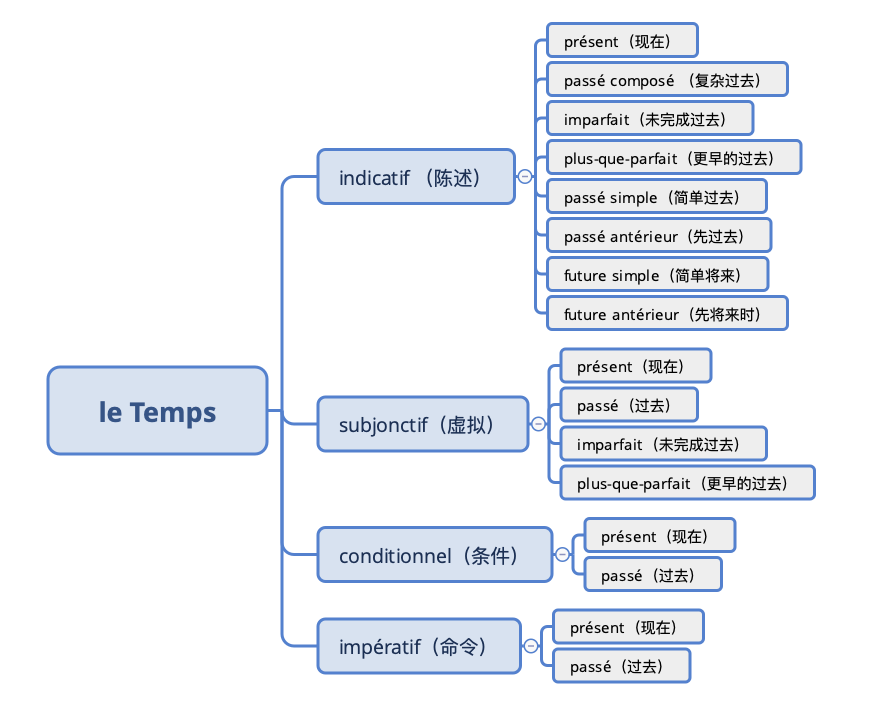
\includegraphics[width=\textwidth]{pic/le-temps}
  \caption{时态}
  \label{fig:le-temps}
\end{figure}


动词变位结尾变化规律如表\ref{tab:congugaison-remember}所示:
\begin{table}[!ht]
  \centering
  \begin{tabular}{p{0.2\textwidth{}}|p{0.2\textwidth{}}|p{0.2\textwidth{}}|p{0.2\textwidth{}}}
    \hline{}
    & \multicolumn{3}{l}{verbe} \\
    \cline{2-4}
    & er & ir & re \\
    \hline
    indicatif présent & e, es, e, ons, ez, ent & is, is, it, issons,
                                                 issez, issent & s, s,
                                                                 t,
                                                                 ons,
                                                                 ez,
                                                                 ent
    \\
    \hline{}
    indicatif passé composé & é & i & u \\
    \hline{}
    indicatif imparfait & \multicolumn{3}{l}{ais, ais, ait, ions, iez,
                          aient} \\
    \hline{}
    indicatif future simple & \multicolumn{3}{l}{ai, as, a, ons, ez,
                              ont} \\
    \hline{}
    subjonctif présent & \multicolumn{3}{l}{e, es, e, ions, eiz, ent}
    \\
    \hline{}
    conditionnel présent & \multicolumn{3}{l}{ais, ais, ait, ions,
                           iez, aient} \\
    \hline{}
  \end{tabular}
  \caption{动词变位助记}
  \label{tab:congugaison-remember}
\end{table}


\begin{itemize}
\item indicatif, inparfait用的présent时态nous的radical
\item indicatif, subjonctif用的présent时态ils的radical
\item conditionnel, présent用的indicatif future simple的radical
\end{itemize}


\begin{itemize}
\item 未完成过去时 用的ai,i,(现在时nous的基)
\item 简单将来时 用的a,ont,(直接加后缀)
\item 虚拟时 用的 e, i (现在时ils的基)
\item 条件时 用的ai, i (将来时的基)
\end{itemize}




%%% Local Variables:
%%% mode: latex
%%% TeX-master: "french"
%%% End:


\chapter{否定(négation)}

\begin{table}[H]
  \centering
  \begin{tabular}[H]{p{0.25\textwidth}||p{0.35\textwidth}|p{0.4\textwidth}}
    \hline{}
    \multirow{2}{8em}{Marque de la négation} & \multicolumn{2}{c}{Place des mqrques de la négation} \\
    \cline{2-3}
                                             & Temps simple & Temps composé \\
    \hline

    (ne) ... pas & (ne) + verbe + pas & (ne) + aux + pas + verbe \\
    (ne) ... plus & (ne) + verbe + plus & (ne) + aux + plus + verbe \\
    (ne) ... rien & (ne) + verbe + rien & (ne) + aux + rien + verbe \\
    (ne) ... jamais & (ne) + verbe + jamais & (ne) + aux + jamais + verbe \\
    (ne) ... nulle part & (ne) + verbe + nulle part & (ne) + aux + verbe + {\color{red}nulle part} \\
    (ne) ... personne & (ne) + verbe + personne & (ne) + aux + verbe + {\color{red}personne}\\
    \hline
    
  \end{tabular}
  
  \caption{La négation}
\end{table}


\begin{itemize}
\item ne ... pas:否定
\item ne ... plus:不再
\item ne ... rien:什么都没有(加强没有的程度)
\item jamais: 从没
\item null part: 没任何部分
\item personne: 没任何人
\end{itemize}




\section{L'example}


Elle ne mange jamais de fromage.

Je ne cherchais personne.

Il n'avait aucun doute sur ses capacités.

Il ne rêve à rien.

Je n'avais jamais pensé à cette possibilité.



\section{Le contraire}


\begin{itemize}
\item personne $\ne$ quelqu'un
\item accun $\ne$ quelque
\item rien $\ne$ quelque chose
\item jamais $\ne$ toujour / déjà
\end{itemize}



\chapter{喜欢程度}


\section{les Questions}
\begin{itemize}
\item Est-ce que tu aimes ...?
\item Tu aimes ...?
\item Aimes-tu ...?
\end{itemize}


\section{les Réponses}

从最喜欢到最讨厌:

\begin{itemize}
\item J'adore 
\item J'aime beaucoup de
\item J'aime
\item Comme-ci, comme-ca
\item Je n'aime pas
\item Je n'aime pas beaucoup de
\item Je déteste
\end{itemize}


%%% Local Variables:
%%% mode: latex
%%% TeX-master: "french"
%%% End:


\chapter{连读(liaison)}
\label{cha:liaison}


\section{什么是连读?}

法语中的连读是:前一个单词结尾的不发音辅音和后一个单词开始的元音连起来读,从
而省略中间的停顿。

为什么会这样呢?
在法语品读规则中,单词结尾的辅音字母一般是不发音的,为了避免元音直接过
渡到元音,因此让本不发音的结尾辅音字母发音,从而更方面的过渡到下一个音。



\section{连读中字母的发音}

在多数情况下,字母的发音就是它本身书写的那个字母的发音,但有如下例外情
况:

\begin{itemize}
\item s [z]
\item d [t]
\item f [v]
\item x [z]
\end{itemize}


\section{什么时候连读}x

连读是和语法想关联的,你只能连读语法上紧密关联的词语(意群)。
连读是为了使意思上紧密关联的词语在声音上也紧密关联。
根据单词在句子中的链接方式,连读可以是必须的、禁止的或可选的。



\subsection{必须的连读}

\subsubsection{名词群}

\begin{itemize}
\item 冠词 + 名词或者形容词 (les amis \textipa{[lE za mi]}, les anciens élèves \textipa{[lE z\~a si j\~E ze lEv]})
\item 数字 + 名词或者形容词 (deux enfants \textipa{[d\o \ z\~a f\~a]})
\item 形容词 + 名词或者形容词 (les anciens élèves \textipa{[lE z\~a si j\~E ze lEv]}, petit ami \textipa{[p@ ti ta mi]})
\end{itemize}


\subsubsection{动词群}

\begin{itemize}
\item 代词 + 代词 (Nous en avons \textipa{[nu z\~a na v\~O]})
\item 代词 + 动词或者形容词 (Nous en avons \textipa{[nu z\~a na v\~O]}, Vous avez \textipa{[nu za ve]})
\end{itemize}

\subsubsection{副词、连词和单音节介词}

bien étrange \textipa{[bj\~E ne tr\~a Z]}

chez elle \textipa{[Se zEl]}

quand on décidera \textipa{[k\~a t\~O de si d@ ra]}

tout entier \textipa{[tu t\~a ti tje]}

très utile \textipa{[trE zy til]}	


\subsubsection{Quand + est-ce que }

Quand + est-ce que \textipa{[k\~a tEsk]}


\subsubsection{固定搭配}

avant hier \textipa{[a v\~a tjEr]}

c’est-à-dire	\textipa{[sE ta dir]}

comment allez-vous ? \textipa{[cO m\~a ta le vu]}

plus ou moins	\textipa{[ply zu mw\~E]}


\subsection{禁止的连读}


\subsubsection{嘘音(aspiré)h前}

en haut \textipa{[\~a o]}

les héros \textipa{[lE e ro]}


\subsubsection{onze和 oui前}

les onze enfants \textipa{[lE O z\~a f\~a]}

deux oui et un non \textipa{[d\o wi e \~a n\~O]}

\subsubsection{人名后}

Robert a 15 ans. \textipa{[rO bEr a k\~E z\~a]}

\subsubsection{单数名词后}

mon chat aime jouer \textipa{[m\~O Sa Em jue]}

un garçon intelligent \textipa{[\~a gar s\~O \~E tE li Z\~a]}


\subsubsection{et后}

un homme et une femme \textipa{[\~a nOm e yn fam]}

\subsubsection{疑问副词和toujours后}

Comment est-elle ?	\textipa{[kO m\~a e  tEl]}

Combien en vois-tu ?	\textipa{[k\~O bj\~E \~a vwa ty]}

Quand aimes-tu étudier ? \textipa{[k\~a Em ty e ty dje]}

toujours aimable  \textipa{[tu Zu rE mabl]}

\subsubsection{倒装后}

A-t-on osé ?	\textipa{[a t\~O o ze]}

Parlez-vous espagnol ?	\textipa{[par le vu E spa \textltailn Ol]}

Ont-elles étudié ?	\textipa{[\~O tE le ty die]}

Vont-ils habiter bien ?	\textipa{[v\~O ti la bi te bj\~E]}

\subsection{可选的连读}

一般来说,当连读是可选的,大多数人选择不连读。




%%% Local Variables:
%%% mode: latex
%%% TeX-master: "french"
%%% End:


\chapter{特殊符号}



\begin{table}[H]
  \centering
  \begin{tabular}{p{0.2\columnwidth}p{0.4\columnwidth}}
    \toprule[2pt]
    \head{symbole} & \head{nom} \\
    \midrule[1.5pt]
    . & point \\
    ç & c cédille \\
    ; & point virgule \\
    , & virgule \\
    - & trait d'union \\
    $\ll$ & guillemet\textipa{[gijmE]} \\
    \# & numero, dièse \\
    / & barre oblique \\
    $\backslash$ &  barre oblique inversée \\
    + & plus \\
    * & astérisque \\
    \_{} & tiret \\
    ' & apostrophe \\
    ë & e tréma \\
    û & u accent circonflexe \\
    @ & arobase \\
    à & a accent grave \\
    é & e accent aigu \\
    \bottomrule[2pt]
  \end{tabular}
  \caption{Symbole}
\end{table}

%%% Local Variables:
%%% mode: latex
%%% TeX-master: "french"
%%% End:



\chapter{基于某个时间节点的时间}

\begin{table}[H]
  \centering
  \begin{tabular}{cc}
    \toprule[1.5pt]
    \keyword{基于现在的时间} & \keyword{基于某个时间节点的时间} \\
    \midrule[1.5pt]{}
    avant-hiver(前天) & avant-veille(前两天) \\
    hier(昨天) & veille(前一天) \\
    aujourd'hui(今天) & ce jour-là(那天) \\
    demain(明天) & lendemain(后一天) \\
    après-demain(后天) & surlendemain(后两天) \\
    \bottomrule[1.5pt]
  \end{tabular}
  \caption{Le temps}
\end{table}
%%% Local Variables:
%%% mode: latex
%%% TeX-master: "french"
%%% End:


\chapter{比较级(le comparatif)}
\label{cha:le-comparatif}


\begin{itemize}
\item plus + adjectif / de nom + que: 比 ... 更
\item moins + adjectif / de nom + que: 不如 ...
\item aussi + adjectif + que / autant + de nom + que: 和 ... 一样
\end{itemize}


例句:
\begin{itemize}
\item J'ai plus de livres que toi.
\item Marie a autant de vêtements que sa mère.
\item Tu as moins de chaussures qu'elle.
\item Cet arbre est plus grand que l’autre.
\item Ta voiture est moins bruyante que la mienne.	
\item Ils sont aussi contents que moi.
\end{itemize}

%%% Local Variables:
%%% mode: latex
%%% TeX-master: "french"
%%% End:


\chapter{形容词的位置(positionnement de l'adjectif)}

形容词\textbf{一般}都放在名词的后面进行修饰的作用,有极少数放在名词的
前面进行修饰,还有一些既可以放在名词的前面也可以放在名词的后面进行修饰,
这种情况统一放名词后面进行修饰就可以了。

\section{放名词前面的形容词}

\textbf{beau, mauvais, bon, grand, gros, petit, haut, vieux, nouveau, jeune,
autre etc}

\begin{itemize}
\item un beau garçon; un bel hôtel; une belle robe;
\item une mauvaise réponse; une bonne réponse;
\item un grand meric; une petite maison;
\item un gros problème; une grosse journée;
\item un autre café svp;
\item un vieux téléviseur; un vieil ordinateur; une vieille machine à café;  
\end{itemize}

\textbf{premier, deuxième, troisième, vingtième, centième, dernier etc}



%%% Local Variables:
%%% mode: latex
%%% TeX-master: "french"
%%% End:


\chapter{宾语代词(pronom complement)}
\label{cha:pronom-complement}

宾语代词的分类如图\ref{fig:pronom-complement}所示。

\begin{figure}[!ht]
  \centering
  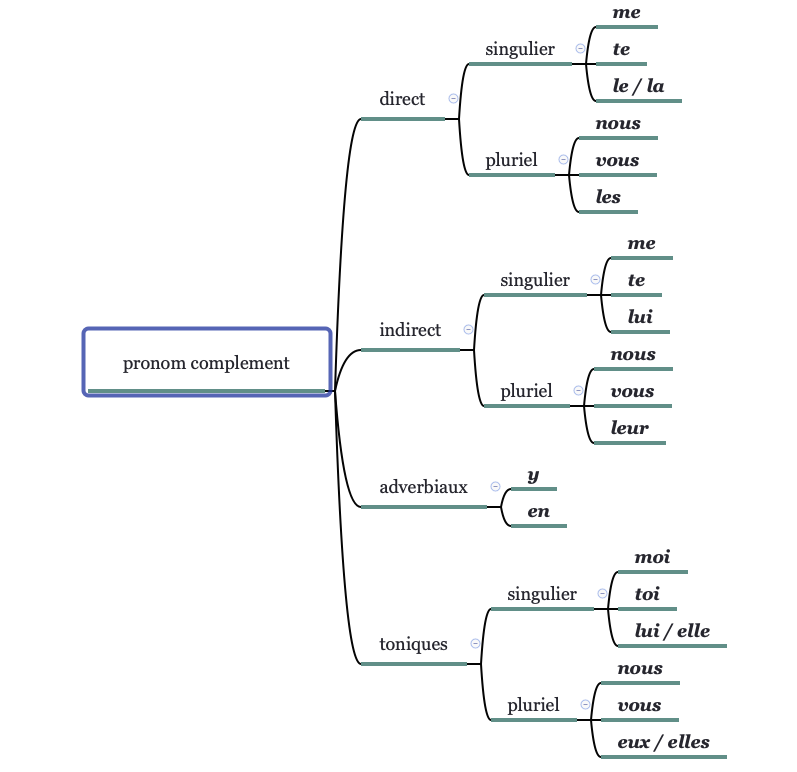
\includegraphics[width=\textwidth]{pic/pronom-complement}
  \caption{pronom complement}
  \label{fig:pronom-complement}
\end{figure}






%%% Local Variables:
%%% mode: latex
%%% TeX-master: "french"
%%% End:


\chapter{名词的阴阳性}

法语中,所有的名词(除了城市)都有阴阳性,对应的,使用的代词(il, elle,
...),形容词(bon, belle, ...),冠词(le, la, un, une)都要使用对应的阴阳性。


\section{人的阴阳性}



一般来说,男的阳性,女的是阴性。

\begin{itemize}
\item un homme
\item un roi
\item une fille
\item une reine
\end{itemize}


当一个单词既可以指代男的,又可以指代女的,往往通过结尾来区别男女(一般
以e结尾的,无变化)。

\begin{itemize}
\item un camarade
\item une camarde
\item un employé
\item une employée
\end{itemize}



\section{动物的阴阳性}


有些是不同的的单词表示阴阳性,un baureau(a bull), une vache(a cow)。
有些是通过改变不同的结尾,un chien, une chienne。
有些不因性别而变化,un poisson。


\section{物体的阴阳性}

没有物理特征来区分名词的阴阳性,但有些规律可以帮助记忆。
\begin{itemize}
\item 以e结尾的一般是阴性
\item 以辅音结尾的,一般是阳性
\item 星期,月份,季节一般是阳性(le lundi)
\item 语言一般是阳性(le français)
\item 大部分的重量和测量一般是阳性(un gramme, un mètre)
\item 从英语引进的词一般为阳性(le football)
\end{itemize}


以下结尾的一般为阳性:
\begin{itemize}
\item age (un village)
\item ment (un appartement)
\item oir (un mirroir)
\item sme (le tourisme)
\item eau (un cadeau)
\item eu (un jeu)
\item ou (le genou)
\item ier (le cahier)
\item in (un magasin)
\item on (un ballon)
\end{itemize}

以下结尾的一般是阴性:
\begin{itemize}
\item ance (la chance)
\item anse (une danse)
\item ence (la patience)
\item ense (la défense)(特例:la silence)
\item ion (une région)
\item té (une spécialité)
\item tié (la moitié) (特例:un été, la pâté)
\end{itemize}



\section{名词阴阳性的转变}
一般是在词尾加e变成阴性,以e结尾的一般不变。


其他规则:
\begin{itemize}
\item f $\rightarrow$ ve (un veuf/une veuve)
\item x $\rightarrow$ se (un époux/une épouse)
\item eur $\rightarrow$ euse (un danseur/une danseuse)
\item teur $teuse/trice$ (un chanteur/une chanteuse, un acteur/une
  actrice)
\item an $\rightarrow$ anne (un paysan/une paysanne)
\item ien $\rightarrow$ ienne (un Parisien/une Parisienne)
\item on $\rightarrow$ onne (un lion/une lionne)
\item er $\rightarrow$ ère (un étranger/une étrangère)
\item et $\rightarrow$ ette (le cadet/la cadette)
\item el $\rightarrow$ elle (un professionnel/une professionnelle)
\end{itemize}

%%% Local Variables:
%%% mode: latex
%%% TeX-master: "french"
%%% End:




\chapter{时间}

\section{Le mois}

\begin{description}
\item[janvier] \textipa{[Z\~avje]} 1
\item[février] \textipa{[fevrije]} 2
\item[mars] \textipa{[mars]} 3
\item[avril] \textipa{[avril]} 4
\item[mai] \textipa{[mE]} 5
\item[juin] \textipa{[Z4\~E]} 6
\item[juillet] \textipa{[Z4ijE]} 7
\item[août] \textipa{[u(t)]} 8
\item[septembre] \textipa{[sEpt\~abr]} 9
\item[octobre] \textipa{[OktObr]} 10
\item[novembre] \textipa{[nOv\~abr]} 11
\item[décembre] \textipa{[des\~abr]} 12
\end{description}


\section{La semaine}

\begin{description}
\item[Lundi] \textipa{[l\~\oe di]} 1
\item[Mardi] \textipa{[mardi]} 2
\item[Mercredi] \textipa{[mErkr@di]} 3
\item[Jeudi] \textipa{[Z\o di]} 4
\item[Vendredi] \textipa{[v\~adr@di]} 5
\item[Samedi] \textipa{[samdi]} 6
\item[Dimanche] \textipa{[dim\~aS]} 7
\end{description}



\section{La saison}

\begin{itemize}
\item Le printemps: spring
\item L’été (m): summer
\item L’automne (m): fall
\item L’hiver (m): winter
\end{itemize}

\section{La journée}
\begin{itemize}
\item le matin: 早晨
\item le midi: 中午
\item le soir: 傍晚
\item la nuit: 夜晚
\item le jour:天

\end{itemize}

%%% Local Variables:
%%% mode: latex
%%% TeX-master: "french"
%%% End:

\backmatter{}


\end{document}

%%% Local Variables:
%%% mode: latex
%%% TeX-master: t
%%% End:
